
本節では、仮想マシンを用いてネットワークとファイアウォールの
設定を行う問題を提示する。
演習環境はVagrant+libvirtをもちいて構築することが出来る。
Vagrant+libvirtは、Ubuntu 18.04だとmkenv/ansibleディレクトリ以下にある
Ansible用のファイルを用いるとインストールすることが出来る。
ただし、講義では演習用の環境を用意するため、Vagrant+libvirtをインストールする必要はない。

演習用のOSはOpenBSDとしている。
OpenBSDはセキュリティが強く意識されたOSであり、
OpenBSDのpfの設定は大変明瞭でわかりやすく、初学者に向いているためである。
pfの設定がわかれば、実際のネットワーク機器の設定も行うことが出来るようになるだろう。

演習環境は、mkenv/vagrant以下にある各ディレクトリ内でvagrantを用いると
構築することが出来る。
例えば、以下のようにすることで問題1の演習環境を構築することが出来る。
\begin{lstlisting}[language=,numbers=none]
$ cd mkenv/vagrant/quiz01
$ vagrant up
\end{lstlisting}
問題1では、3つのノードがあるが、そのうちのノードh1へログインしたいときは下記のように入力すると
ログインできる。
\begin{lstlisting}[language=,numbers=none]
$ vagrant ssh h1
\end{lstlisting}
他のノードへログインしたい場合は、一旦h1から抜けて、同じようにh2やh3へとログインすれば良い。
もしも問題をとき終わって環境を破棄したくなったり、設定をミスってしまってもう演習環境を
初期状態に戻したい場合は、destroyで破棄することが出来る。
\begin{lstlisting}[language=,numbers=none]
$ vagrant destroy
\end{lstlisting}
いらなくなった環境は、そのまま放って置くとディスクスペースを圧迫するため、必要なくなったら削除しておこう。

ソースコード~\ref{src:vagrantfile}は、問題1の環境を構築するためのVagrantfileである。
VagrantはRubyによって実装されおり、Vagrantfileというスクリプトで環境設定を記述する。
この設定ファイルでは、仮想マシンにOpenBSD version 6を利用した、h1、h2、h3というホストを用意することが
記述されている。また、L2ネットワークは、q01\_a、q01\_bという2つのネットワークを利用するようにしている。
\begin{lstlisting}[language=Ruby,caption=演習問題1のVagrantfile,label=src:vagrantfile]
Vagrant.configure("2") do |config|
  config.vm.box = "generic/openbsd6"

  config.vm.define :h1 do | h1 |
    h1.vm.hostname = "h1"
    h1.vm.network "private_network", ip: "172.16.0.10", libvirt__domain_name: "q01_a"
  end

  config.vm.define :h2 do | h2 |
    h2.vm.hostname = "h2"
    h2.vm.network "private_network", ip: "172.16.0.20", libvirt__domain_name: "q01_a"
    h2.vm.network "private_network", ip: "172.20.0.20", libvirt__domain_name: "q01_b"
  end

  config.vm.define :h3 do | h3 |
    h3.vm.hostname = "h3"
    h3.vm.network "private_network", ip: "172.20.0.30", libvirt__domain_name: "q01_b"
  end
end
\end{lstlisting}


\subsection{問題1:3ノードの単純なネットワーク}

図~\ref{fig:quiz01}のようなネットワークがあるとする。
このとき、ノードh1からノードh3へ及び、ノードh3からノードh1へIPv4パケットが到達するように、
ノードh1〜h3を設定せよ。ただし、ブリッジ接続ではなく、
ルーティングテーブルを設定してL3レベルでの設定を行うこと。
ヒント:ノードh1〜h3のルーティングテーブルをrouteコマンドで設定し、
ノードh2をIPv4のフォワーディングを行うようにsysctlコマンドで設定せよ。

\begin{figure}
    \centering
    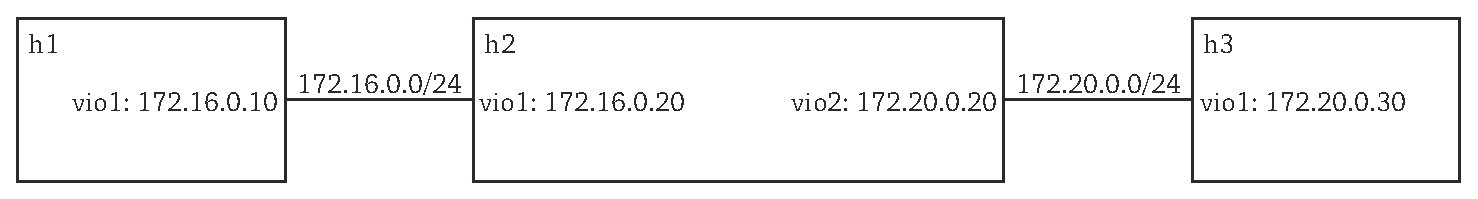
\includegraphics[width=15cm,pagebox=artbox]{figs/quiz01.pdf}
    \caption{問題1:ルーティング実験の3ノードトポロジ図} \label{fig:quiz01}
\end{figure}

\subsection{問題2:4ノードのネットワーク}

図~\ref{fig:quiz02}のようなネットワークがあるとする。
このとき、各ノードから全てのノードへIPv4パケットが到達するように、
ノードh1〜h4を設定せよ。
ただし、ブリッジ接続ではなく、
ルーティングテーブルを設定してL3レベルでの設定を行うこと。

\begin{figure}
    \centering
    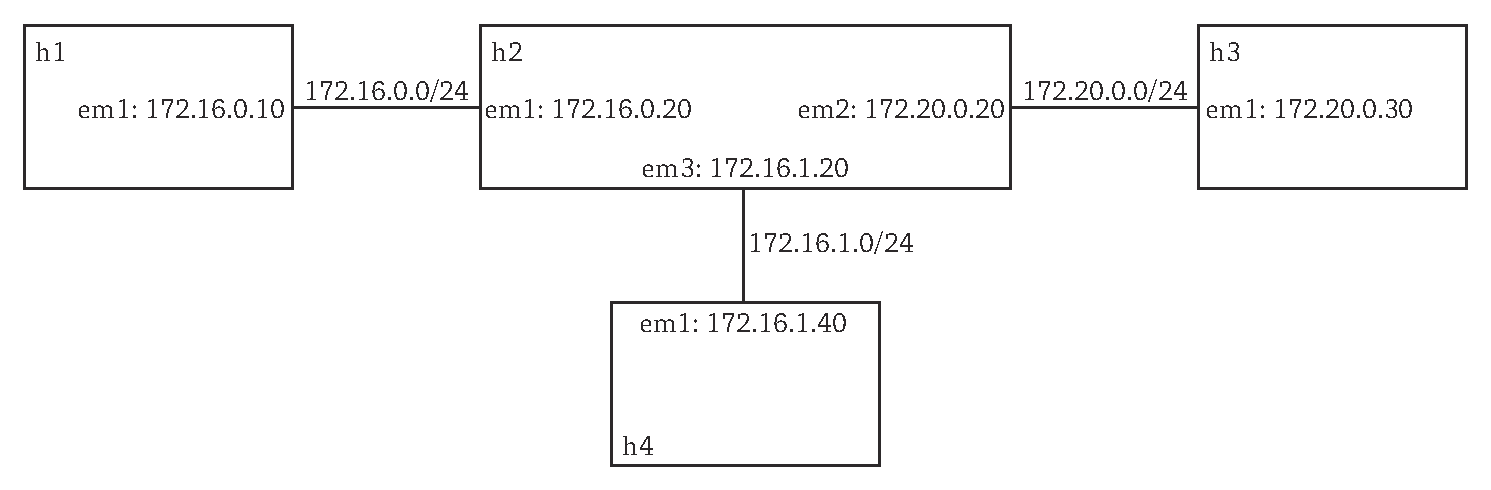
\includegraphics[width=15cm,pagebox=artbox]{figs/quiz02.pdf}
    \caption{問題2および3:ルーティング実験、DMZ実験の4ノードトポロジ図} \label{fig:quiz02}
\end{figure}

\subsection{問題3:DMZ(DeMilitarized Zone)}

同じく、図~\ref{fig:quiz02}のネットワークを利用して、以下の要求を満たすように
サービスを構築し、ノードh2にpfでファイアウォールを構築せよ。
ファイアウォールの設定後は、ping、curlコマンドなどを利用して設定が要求どおりとなっているか確認すること。

\begin{itemize}
    \item ノードh1の所属するネットワーク172.16.0.0/24を社内ネットワークとする
    \item ノードh3の所属するネットワーク172.16.20.0/24をインターネットに接続するための対外ネットワークとする
    \item ノードh4の所属するネットワーク172.16.1.0/24を対外向けサービスを設置するためのDMZネットワークとする
    \item ノードh1、h3、h4にWebサーバを構築せよ
    \item 社内ネットワークから対外ネットワーク及びDMZネットワークへのTCP、UDP、ICMP接続が可能
    \item DMZネットワークから社内ネットワークへのTCP、UDP、ICMP接続は禁止
    \item DMZネットワークから対外ネットワークへのTCP、UDP、ICMP接続は可能
    \item 対外ネットワークからDMZネットワークへの接続はWebのみ可能
    \item 対外ネットワークから社内ネットワークへのTCP、UDP、ICMP接続は禁止
    \item 社内ネットワークとDMZから対外ネットワークへむけて、ソースIPアドレスを詐称してパケットを送信することは禁止
\end{itemize}

\subsection{問題4:ブリッジ}

\begin{figure}
    \centering
    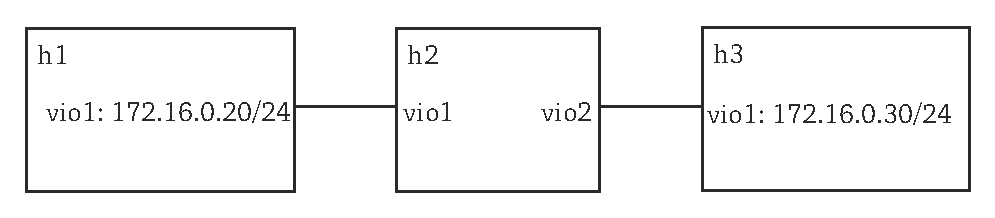
\includegraphics[width=10cm,pagebox=artbox]{figs/quiz04.pdf}
    \caption{問題4:ブリッジ実験のトポロジ図} \label{fig:quiz04}
\end{figure}

図~\ref{fig:quiz04}のネットワークがあるとする。
このとき、ノードh2でブリッジ設定、ノードh1とh3を互いに通信できるようにせよ。
ヒント:ブリッジの設定はifconfigコマンドで行える。

\subsection{問題5:VLAN}

\begin{figure}
    \centering
    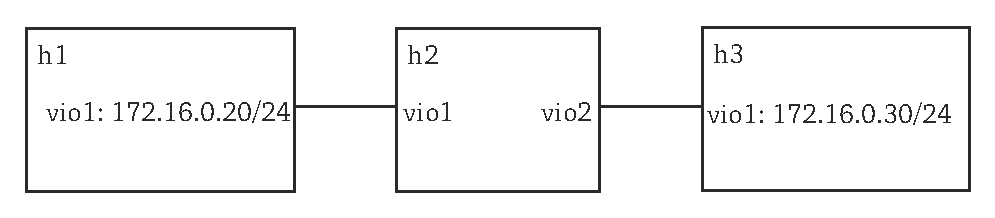
\includegraphics[width=15cm,pagebox=artbox]{figs/quiz05.pdf}
    \caption{問題5:VLAN実験のトポロジ図} \label{fig:quiz05}
\end{figure}

図~\ref{fig:quiz06}のネットワークがあるとする。
このとき、リンクAとA'が同じセグメントに、また、リンクBとB'が同じセグメントとなるように、
タグVLANとブリッジの設定をノードh2、h3、h4で行え。
ヒント:タグVLANとブリッジの設定はifconfigコマンドで行える。

\subsection{問題6:NAPT}

問題3のネットワーク設定を改変し、社内ネットワークから対外ネットワークへの接続はNAPTで接続するように修正せよ。